\fancypagestyle{plain}{\fancyhead{}\renewcommand{\headrulewidth}{0pt}}
\chapter{Esperimenti}
Una volta ultimata l’implementazione del codice, ora più facilmente fruibile grazie alla creazione del file \textit{.lib}, il passo successivo è stato lo sviluppo di applicazioni vere e proprie che potessero fare affidamento sulla libreria Edge Engine. In particolare, in questo capitolo verranno trattati tre esperimenti differenti: il primo riguarderà un esempio di utilizzo su PC Windows (più completo e significativo rispetto a quello descritto nella sezione \ref{prova}, il secondo verterà invece sulla creazione di un plugin per poter usufruire della libreria anche in ambiente Unity3D e, infine, il terzo descriverà un vero e proprio caso applicativo portato a termine da due tesisti triennali del corso di Ingegneria Elettronica e Tecnologie dell'Informazione dell'Università degli Studi di Genova.
\section{Applicazione Windows}
L'esempio di utilizzo per Windows è stato creato al fine di mostrare e testare tutte le potenzialità offerte dall'incremento delle piattaforme supportate da Edge Engine.\\
Come accennato brevemente nella sezione \ref{prova}, in primo luogo è necessario riportare sul Cloud la descrizione della risorsa che si intende adottare. Più in particolare, sono da specificare i parametri mostrati nella tabella seguente:
\begin{table}[H]
	\begin{tabular}{|p{0.15\textwidth}|p{0.44\textwidth}|p{0.32\textwidth}|}
		\hline
		\textbf{Parametri} & \textbf{Nome} & \textbf{URL}\\
		\hline
		\textbf{Thing} & my-pc & {{url}}/v1/things/my-pc\\
		\hline
		\textbf{Feature} & total-ram, total-rom, available-ram, available-rom & {{url}}/v1/features\\
		\hline
		\textbf{Device} & pc-probe & {{url}}/v1/devices/pc-probe\\	
		\hline
		\textbf{Script} & total-rom-installed, total-ram-installed, ram-available, rom-available, average-hourly-available-ram, ram-available-to-mb, rom-available-to-mb,  max-available-ram, max-available-rom & {{url}}/v1/scripts\\	
		\hline
	\end{tabular}
\\\\url = \url{http://students.atmosphere.tools/}
	\caption{Parametri Measurify}
	\label{paramMeas}
\end{table}
Il device \textit{pc-probe} contiene all'interno della sua descrizione le features e gli script ad esso associati. Le prime indicano le grandezze fisiche misurabili dal dispositivo, mentre i secondi rappresentano le funzioni di elaborazione che è possibile applicare ai dati ricevuti. \\
La tabella \ref{script} mostra la struttura degli script implementati. Essi sono composti da due campi principali: \textit{\_id} e \textit{code}.  \textit{\_id} specifica il nome associato allo script stesso, mentre  \textit{code} contiene le effettive operazione che il dispositivo fisico andrà ad effettuare. 
\begin{table}[H]
	\begin{tabular}{|p{0.27\textwidth}|p{0.67\textwidth}|}
		\hline
		\textbf{\_id} & \textbf{code} \\
		\hline
		ram-available & available-ram().send()\\
		\hline
		rom-available & available-rom().send()\\
		\hline
		total-ram-installed & total-ram().send()\\
		\hline
		total-rom-installed & total-rom().send()\\
		\hline
		max-available-ram & available-ram(10).max().send()\\	
		\hline
		max-available-rom & available-rom(10).max().send()\\
		\hline	
		ram-available-to-mb & available-ram().map(a*1024).send()\\
		\hline
		rom-available-to-mb & available-rom().map(a*1024).send()\\
		\hline
		average-hourly-available-ram & available-ram(6m).window(+,0,10).map(a/10).send()\\
		\hline
	\end{tabular}
	\caption{Gli script correlati al device \textit{pc-probe}}
	\label{script}
\end{table}
Prendendo ad esempio lo script \textit{ram-available-to-mb}, il codice in oggetto permette di ricavare la quantità, espressa in gigabyte, di memoria disponibile tramite l’operazione \textit{available-ram()}, la quale viene poi concatenata a \textit{map(a*1024)} che converte il valore ottenuto in megabyte moltiplicandolo per 1024. Infine, tramite la \textit{send()} il campione appena elaborato viene inviato a Measurify.\\
Lo script \textit{average-hourly-available-ram}, invece, calcola la media oraria di ram disponibile, ma necessita di un tempo di elaborazione più lungo di una singola esecuzione dell'engine, come specificato dal codice:\\ \texttt{available-ram(6m).window(+,0,10).map(a/10).send()}\\ L’operazione \textit{available-ram(6m)} permette di campionare ogni sei minuti. Tramite la \textit{window(+,0,10)} poi, viene presa una finestra di dieci input e calcolata la somma di tali elementi. Il calcolo della media viene poi portato a termine grazie alla \textit{map(a/10)}, che opera una divisione sul totale per il numero di campioni presi in considerazione. Infine, il risultato viene inviato al Cloud grazie alla \textit{send()}.\\ 
Una volta riportata sul Cloud la descrizione della risorsa di cui si intende usufruire, è possibile passare allo sviluppo del codice dell'applicazione. Si hanno nuovamente due funzioni principali, \textit{setup} e \textit{action}, che svolgono gli stessi task di autenticazione, elaborazione e invio dei dati descritti nella sezione \ref{prova}. In questo caso però, \textit{action} viene eseguita ciclicamente per un numero di volte specificato dalla variabile \textit{loopCount}. Questo al fine di poter disporre di un tempo di esecuzione più lungo, nel caso in cui si desideri, ad esempio, usufruire dello script \textit{average-hourly-available-ram}, il quale richiede un'ora di tempo per collezionare i campioni.\\
Inoltre, al fine di recuperare dalla macchina in uso le informazioni relative all'utilizzo delle memorie RAM e ROM, sono state implementate le funzioni \textit{getRAMinfo} e  \textit{getROMinfo}. Esse sono esclusive per piattaforme dotate di sistema operativo Windows in quanto fanno uso della libreria proprietaria. Qualora si riveli necessario modificare il progetto al fine di adattarlo ad altri OS, sarà sufficiente sostituire le suddette funzioni con altre, specifiche del target desiderato.\\
Un esempio di dato elaborato dallo script \textit{ram-available-to-mb} del device \textit{my-pc} e conservato sul Cloud è mostrato in figura \ref{datowin}.
\begin{figure}[H]
	\centering
	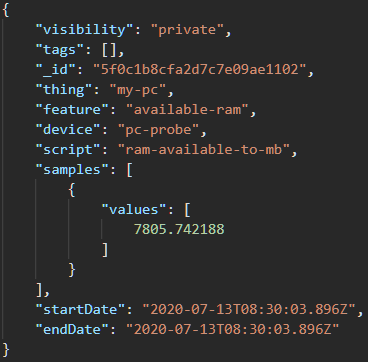
\includegraphics[scale=0.7]{pics/datowin}
	\caption{Dato relativo al valore di memoria RAM disponibile convertito in MB e conservato sul Cloud}
	\label{datowin}
\end{figure}

